\chapter{Realizzazione del tool}

Il codice sorgente Javascript in input viene processato attraverso diverse fasi, in sequenza: parsing, creazione del control flow graph o cfg, analisi, presentazione dei risultati.

\section{Parsing}

Il parsing viene fatto per mezzo della libreria open source Mozilla Rhino. Il risultato del parsing di Rhino è un albero sintattico concreto. Questo viene convertito nell'albero sintattico astratto definito nel package \texttt{it.univr.jsanalyzer.ast}, e i cui componenti sono presenti in \texttt{it.univr.jsanalyzer.builder}.

Tutti gli alberi sintattici e tutti i grafi definiti all'interno del progetto si appoggiano sulle classi della libreria open source GraphStream. Il suo utilizzo ci permette di non \emph{reinventare la ruota}. Inoltre la libreria offre diversi metodi per la visualizzazione dei grafi. 

\section{Componenti dell'albero sintattico astratto}

Ogni nodo dell'albero astratto è uno \texttt{Statement}. Questo rappresenta un'istruzione generica, una linea di codice. La struttura di questo componente è una classe astratta, che viene ereditata e completata dalle classi concrete che rappresentano le istruzioni specifiche (dichiarazione, assegnamento, selezione, ...). 

Le guardie booleane e i valori a destra dell'assegnazione sono \texttt{Expression}. Queste sono definite ricorsivamente attraverso le classi \texttt{UnaryExpression}, \texttt{Binary\-Expression} e \texttt{*Literal}. In casi eccezionali, un'istruzione può essere sia uno Statement che un'Expression, per esempio un'assegnamento che compare all'interno di un'espressione: \mintinline{javascript}{var result = 3 * (a = b)}.

Ad ogni Statement è assegnato un identificatore univoco all'interno dell'albero sintattico. Questo è chiamato \texttt{AbstractPoint} ed è una coppia di interi: \emph{linea di codice} ed \emph{offset}. L'offset è non-zero solo quando lo Statement compare all'interno dell'espressione. All'interno delle espressioni tutti gli Statement vengono enumerati e ad ognuno viene assegnato l'AbstractPoint con la stessa linea ma offset che viene di volta in volta incrementato. Trovi un esempio in Figura~\ref{fig:realizzazione:label-hierarchy}.

\begin{figure}[htbp]
    \centering
    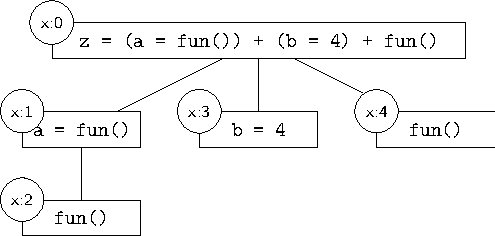
\includegraphics[width=0.5\textwidth]{scheme-generator/generated/label-hierarchy.pdf}
    \caption{\texttt{AbstractPoint} di un'istruzione alla linea $x$}
    \label{fig:realizzazione:label-hierarchy}
\end{figure}

\section{Control flow graph}

La classe \texttt{ControlFlowGraph} si occupa della costruzione del control flow graph a partire dall'albero sintattico astratto. Questa si appoggia sulla classe \texttt{MultiGraph} della libreria GraphStream anche per la visualizzazione. Sono possibili diversi \emph{layout} di visualizzazione a schermo, tra cui il layout gerarchico pensato appositamente per la presentazione del codice.

\section{Interprete}

L'interprete prende in input un control flow graph di Statement da eseguire. L'esecuzione si appoggia su una struttura ausiliaria detta \texttt{AbstractState} che sarà anche il risultato dell'operazione. 

L'interprete esegue anche in modo non deterministico le istruzioni del cfg aggiornando l'AbstractState. La classe \texttt{AbstractInterpreter} è incompleta, ed esegue le operazioni su oggetti astratti \texttt{AbstractValue}. Il programmatore dovrà definire il suo dominio di oggetti che ereditano da AbstractValue, le operazioni tra questi oggetti (i cui metodi sono elencati nella classe \texttt{AbstractDomainOperation}). Questi saranno poi passati al costruttore della classe AbstractInterpreter.

\subsection{\texttt{AbstractValue}}

L'interfaccia \texttt{AbstractValue} funge da segnaposto all'interno dei metodi che lavorano su oggetti del dominio astratto non ancora specificato. Un esempio di classi che la implementano sono \texttt{Top} e \texttt{Bottom}. 

Il programmatore specificherà poi il dominio sul quale vorrà lavorare. Noi utilizziamo per l'analisi il dominio SEA descritto in \cite{arceri}.

\subsection{\texttt{AbstractDomainOperation}}

L'interfaccia \texttt{AbstractDomainOperation} rappresenta una serie di operazioni che devono effettuare gli elementi del dominio. Una volta specificate le classi del dominio (es. SEA), dovrò creare una classe che implementa \texttt{AbstractDomainOperation} e che lavora in simbiosi con il dominio specificato.

\subsection{\texttt{AbstractState}}

La classe \texttt{AbstractState} rappresenta lo stato della computazione in ogni suo punto del codice. Il suo elemento principale è la classe \texttt{AbstractEnvironment}, cioè uno screenshot della memoria in un certo punto del codice (ad una certa linea, con una certa \emph{CallString} - vedi Sezione~\ref{sec:callstring}). L'\texttt{AbstractState} è quindi una mappa che associa ad una coppia $\struct{\ell, cs}$ un certo \texttt{AbstractEnvironment}.

\begin{figure}[htbp]
    \centering
    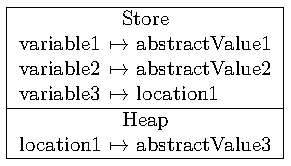
\includegraphics{scheme-generator/generated/environment.pdf}
    \caption{Struttura dell'\texttt{AbstractEnvironment}}
    \label{fig:realizzazione:abstractenvironment}
\end{figure}

L'\texttt{AbstractEnvironment} è formato da due strutture:
\begin{itemize}
    \item \texttt{AbstractStore}: mappa del tipo \texttt{Variable}$\mapsto$\texttt{AbstractValue} dove \texttt{Variable} è l'oggetto che denota una variabile; contiene le variabili globali e locali non allocate dinamicamente;
    \item \texttt{AbstractHeap}: mappa del tipo \texttt{AbstractLocation}$\mapsto$\texttt{AbstractValue} dove \texttt{AbstractLocation} è l'oggetto che denota un puntatore ad un oggetto.
\end{itemize}

\subsection{Dominio SEA}

Il dominio SEA utilizzato nella nostra analisi è formato da questi elementi:
\begin{itemize}
    \item \texttt{Interval}: intervallo di interi a 64-bit più due valori speciali $+\infty$ e $-\infty$;
    \item \texttt{Bool}: uno sei valori \texttt{TRUE}, \texttt{FALSE}, \texttt{UNKNOWN};
    \item \texttt{FiniteAutomata}: stringhe rappresentate come automi a stati finiti.
\end{itemize}
Oltre a questi elementi è presente anche la classe \texttt{AbstractObject} che fa parte come \texttt{AbstractValue} del dominio generico ed è comune a tutti i domini specificati dal programmatore. L'\texttt{AbstractObject} è una mappa di variabili in valori che implementa il concetto di proprietà dell'oggetto (Sezione~\ref{sec:js:createobj}). 

\subsection{Dichiarazioni ed assegnamenti}\label{sec:realizzazione:dichiarazioni}
\begin{javascriptcode}
var x = 2;
x = x + 2;
\end{javascriptcode}
La prima istruzione è una dichiarazione. Questa aggiunge la variabile \texttt{x} all'ambiente (Store) ed il suo valore astratto, considerando il dominio descritto precedentemente, è l'intervallo $[2,2]$ (cioè esattamente 2). L'ambiente modificato viene assegnato all'istruzione successiva \texttt{2:0}. Questa è un assegnamento, e modifica la variabile precedentemente dichiarata. L'ambiente che ne risulta viene assegnato ad \texttt{EOF}. 

\begin{figure}[htbp]
    \centering
    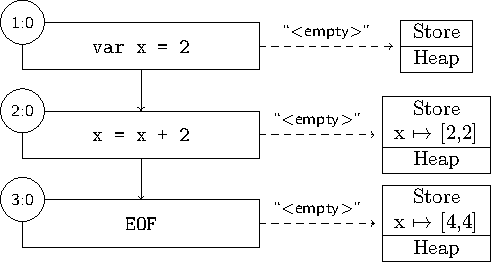
\includegraphics{scheme-generator/generated/example-declaration.pdf}
    \caption{Esempio della Sezione~\ref{sec:realizzazione:dichiarazioni}}
    \label{fig:realizzazione:dichiarazioni}
\end{figure}

Il risultato dell'esecuzione del codice sopra è visibile in Figura~\ref{fig:realizzazione:dichiarazioni}. Gli \texttt{AbstractEnvironment} delle istruzioni sono visibili a lato e connessi a queste tramite frecce tratteggiate. L'etichetta sulla freccia tratteggiata è chiamata \emph{call string} ed il suo significato può essere ignorato per il momento e verrà spiegato nella Sezione~\ref{sec:callstring}.

\subsection{Selezione}\label{sec:realizzazione:selezione}
\begin{javascriptcode}
var x = ..., y = 10; // x = 0 oppure x = 1
if(x == 0) {
    y = 5;
    x = y + 1;
} else {
    y = 33;
    x = y + 2;
}
\end{javascriptcode}
L'esecuzione del costrutto \texttt{if} parte con la valutazione della guardia. Se la guardia è sicuramente vera o sicuramente falsa, procediamo eseguendo la giusta diramazione. Quando non sappiamo con certezza questa cosa, dobbiamo eseguire separatamente.

\begin{figure}[htbp]
    \centering
    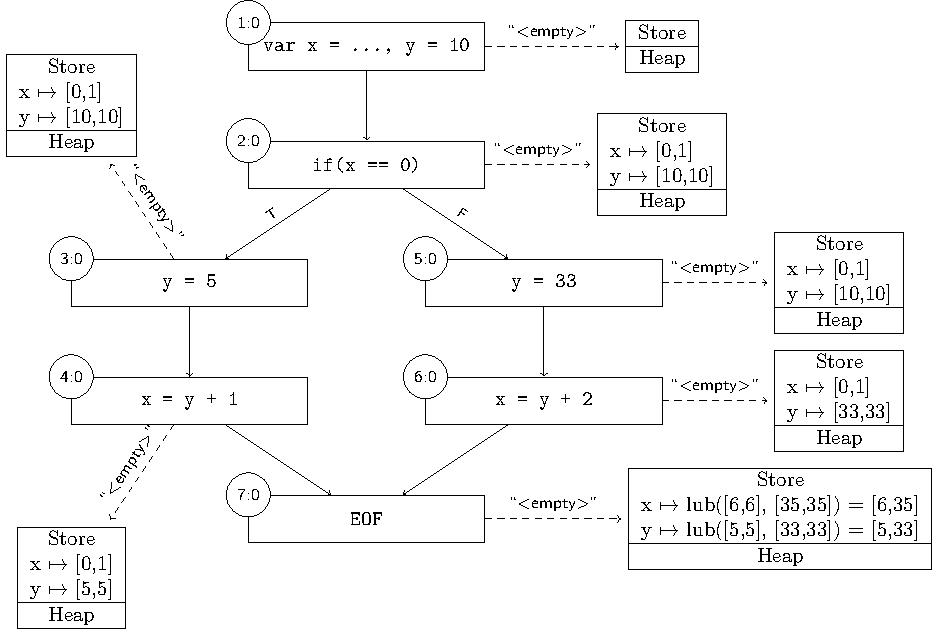
\includegraphics[width=\textwidth]{scheme-generator/generated/example-if.pdf}
    \caption{Esempio della Sezione~\ref{sec:realizzazione:selezione}}
    \label{fig:realizzazione:selezione}
\end{figure}

Nel codice sopra, quando valutiamo la guardia \texttt{x==0} questa potrebbe essere sia vera che falsa. Allora eseguiamo il branch ``vero" e ne mettiamo normalmente e ci salviamo a parte l'ambiente dopo aver eseguito l'ultima istruzione del branch ($e_1$). Eseguiamo poi allo stesso modo il branch ``falso" e, come per il precedente, mettiamo da parte l'ambiente dopo aver eseguito l'ultima istruzione del branch ($e_2$). L'ambiente della prima istruzione dopo il costrutto di selezione sarà $\join[e_1][e_2]$. 
Gli ambienti che risultano dall'esecuzione sono visibili in Figura~\ref{fig:realizzazione:selezione}.

\subsection{Iterazione}\label{sec:realizzazione:iterazione}
\begin{javascriptcode}
var x = 1;
while (x <= 3) {
    x = x + 1;
}
\end{javascriptcode}
Il costrutto \texttt{while} viene eseguito come segue parte con la valutazione della guardia. Se questa è falsa si continua con l'istruzione successiva. Altrimenti si esegue il corpo del while. Alla successiva iterazione, se la guardia potrebbe ancora essere vera, si esegue il widening del vecchio ambiente con il nuovo. Nel caso si raggiunga il fixpoint si continua con l'esecuzione, altrimenti si itera ancora. Gli ambienti che risultano dall'esecuzione sono visibili in Figura~\ref{fig:realizzazione:iterazione}.

\begin{figure}[htbp]
    \centerfloat
    \begin{subfigure}{.8\linewidth}
        \centering
        \fbox{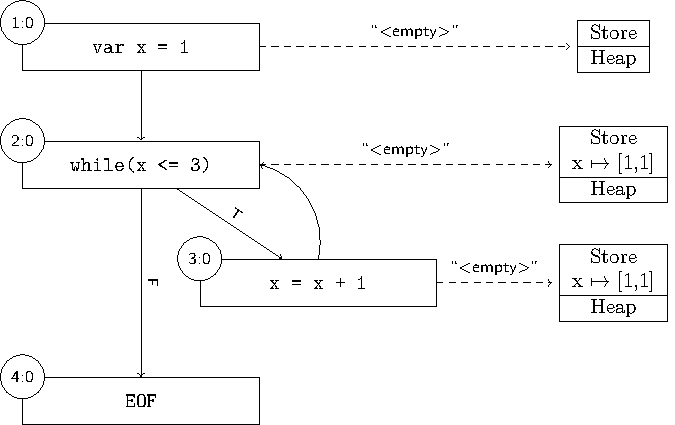
\includegraphics[width=0.8\textwidth]{scheme-generator/generated/example-while-1.pdf}}
        \caption{Prima iterazione}
        \label{fig:realizzazione:while-2}
    \end{subfigure}%
    \begin{subfigure}{.8\linewidth}
        \centering
        \fbox{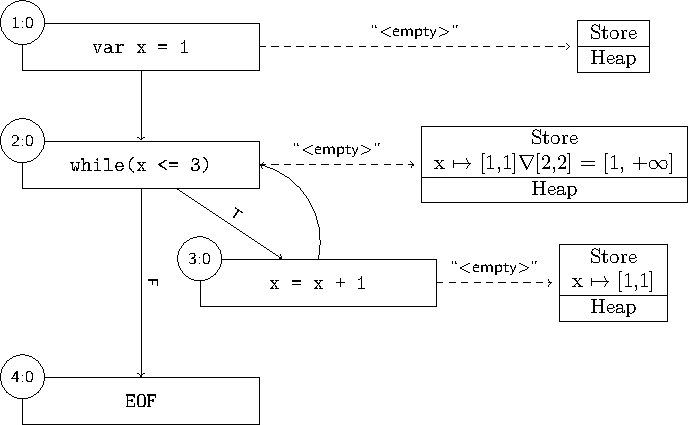
\includegraphics[width=0.8\textwidth]{scheme-generator/generated/example-while-2.pdf}}
        \caption{Seconda iterazione}
        \label{fig:realizzazione:while-2}
    \end{subfigure}\\[4ex]
    \begin{subfigure}{.8\linewidth}
        \centering
        \fbox{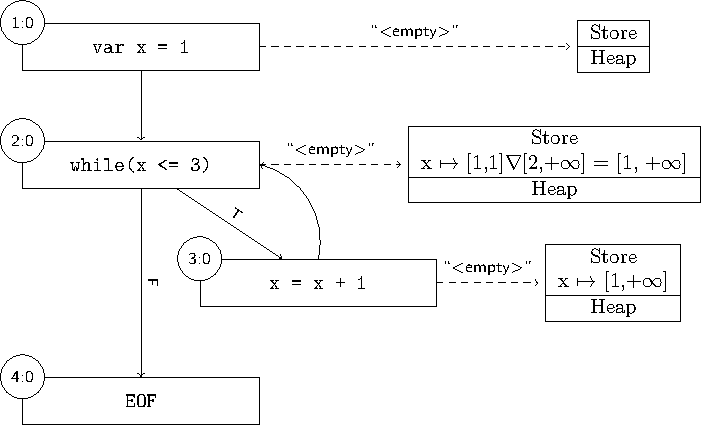
\includegraphics[width=0.8\textwidth]{scheme-generator/generated/example-while-3.pdf}}
        \caption{Terza iterazione}
        \label{fig:realizzazione:while-2}
    \end{subfigure}%
    \begin{subfigure}{.8\linewidth}
        \centering
        \fbox{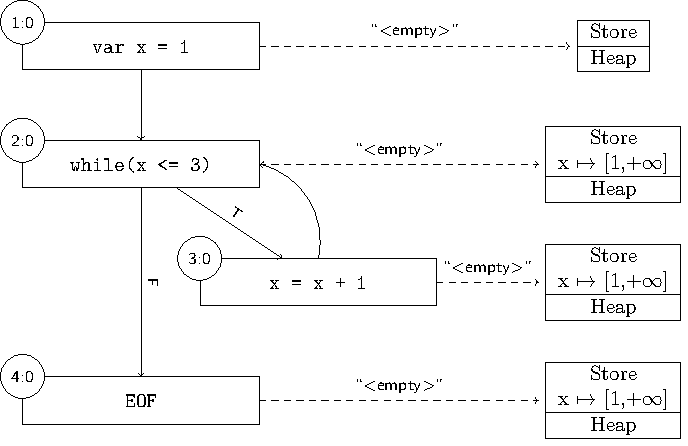
\includegraphics[width=0.8\textwidth]{scheme-generator/generated/example-while-4.pdf}}
        \caption{Completo}
        \label{fig:realizzazione:while-2}
    \end{subfigure}%
    \caption{Esempio della Sezione~\ref{sec:realizzazione:iterazione}}
    \label{fig:realizzazione:iterazione}
\end{figure}

\subsection{Chiamate a funzione}\label{sec:callstring}

Ogni funzione è definita da un control flow graph con una prima istruzione segnaposto detta \emph{entry point} ed un'ultima istruzione segnaposto detta \emph{exit point}.

Quando incontro la definizione di funzione, questa viene aggiunta all'ambiente in tre passi:
\begin{enumerate}
    \item aggiungo allo store un binding di tipo \emph{nome funzione} $\mapsto$ \emph{insieme di locazioni}, dove ogni locazione è un riferimento ad un oggetto nell'heap; se è già presente un binding con chiave \emph{nome funzione} allora passo al punto successivo;
    \item genero una locazione per un oggetto \texttt{AbstractFunction} che conterrà la definizione della funzione incontrata; aggiungo all'heap un binding di tipo \emph{locazione} $\mapsto$ \emph{definizione di funzione};
    \item aggiungo allo store, all'entry di chiave \emph{nome funzione}, la locazione generata nel punto precedente al corrispondente insieme di locazioni.
\end{enumerate}

Quando incontro la chiamata a funzione connetto \emph{dinamicamente} la chiamata agli entry point ed exit point della funzione. Prima della chiamata valuto gli argomenti della funzione. Alla funzione passo poi l'ambiente nel punto precedente della chiamata più gli argomenti valutati all'\emph{entry point}. Al termine della chiamata ritorna un valore. 

\subsubsection{Chiamata a funzioni na\"ive} 

Eseguiamo le funzioni come se fossero un normale pezzo di codice. Con questo metodo ad ogni chiamata di funzione possiamo perdere precisione. Viene introdotto il metodo delle CallString.

\subsubsection{Chiamata a funzione con call string}\label{sec:callstring:internal}
\begin{javascriptcode}
function add(n,m) {
    return n + m;
}
var x = add(1000, 1);
var y = add(-500, 1);
\end{javascriptcode}
Il metodo delle call string permette di aumentare la precisione delle chiamate a funzione. Occorre differenziare gli ambienti delle istruzioni della funzione a seconda di chi l'ha chiamata.

Le chiamate vengono identificate grazie all'identificatore che hanno le istruzioni, visibile all'interno degli schemi nel cerchio alla loro destra. L'identificatore dell'istruzione è ovviamente univoco.

\begin{figure}[htbp]
    \centering
    \begin{subfigure}{\linewidth}
        \centering
        \fbox{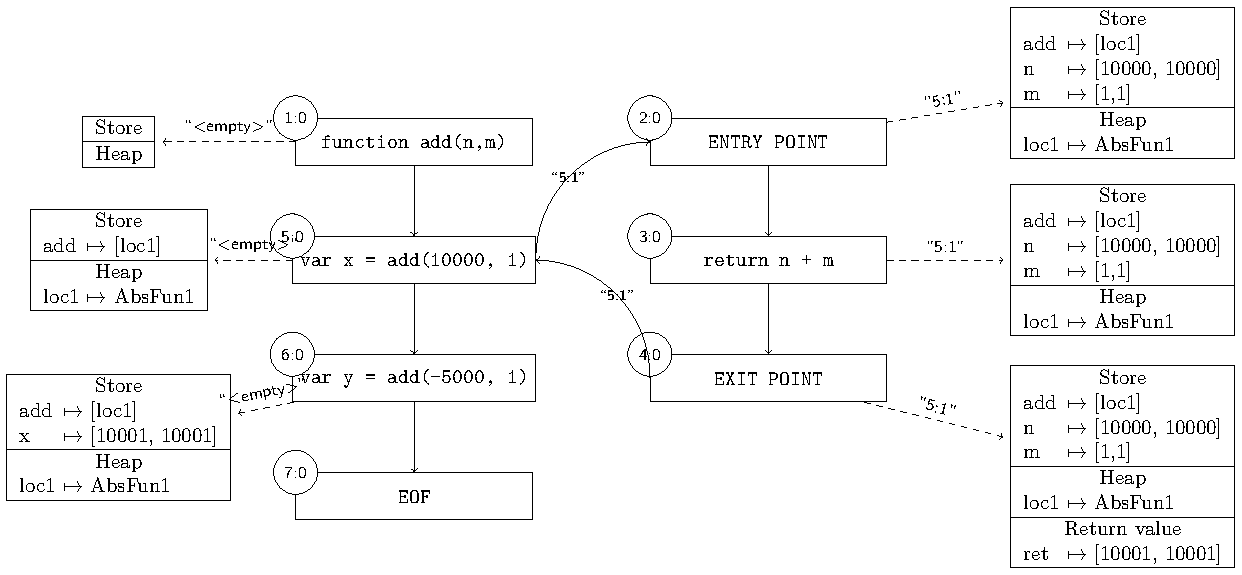
\includegraphics[width=\textwidth]{scheme-generator/generated/example-fun-cs-1.pdf}}
        \caption{Dopo la prima chiamata}
    \end{subfigure}\\[4em]
    \begin{subfigure}{\linewidth}
        \centering
        \fbox{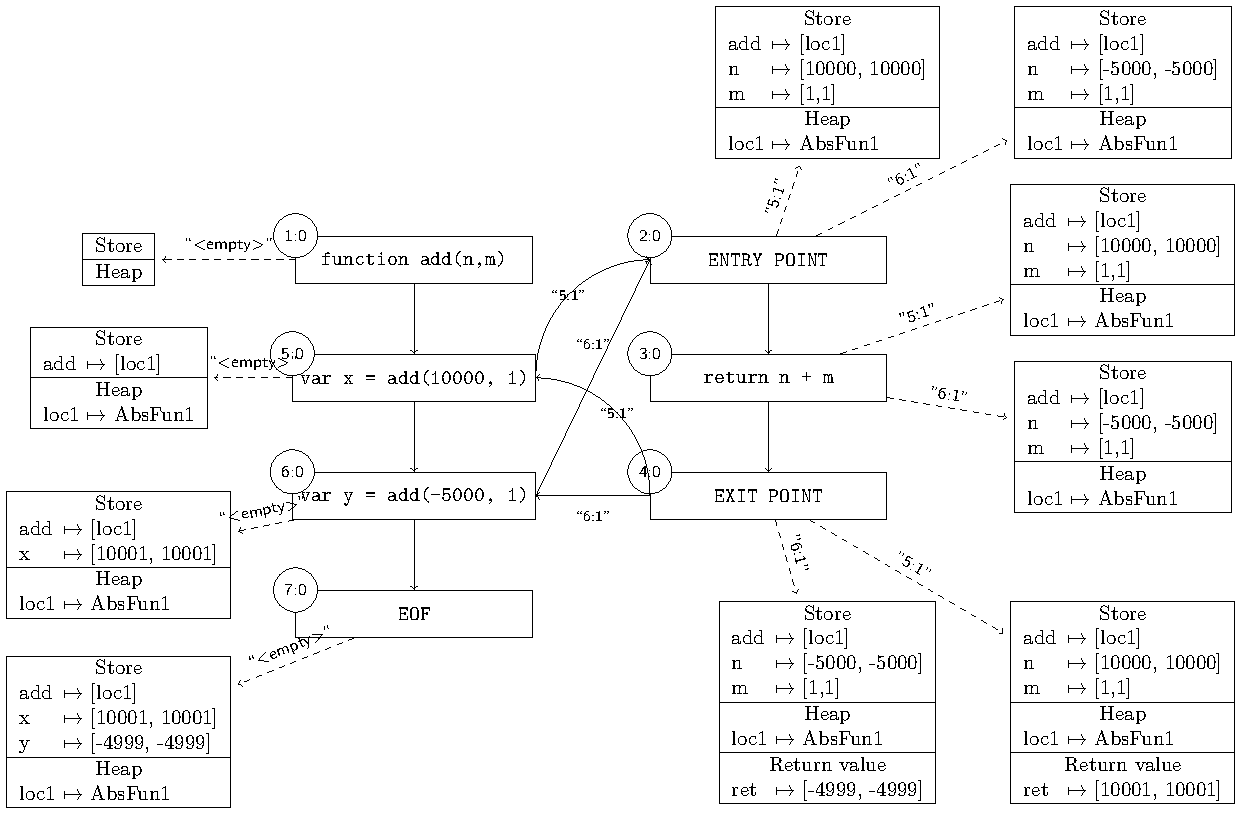
\includegraphics[width=\textwidth]{scheme-generator/generated/example-fun-cs-2.pdf}}
        \caption{Dopo la seconda chiamata}
    \end{subfigure}
    \caption{Esempio della Sezione~\ref{sec:callstring:internal}}
    \label{fig:realizzazione:callstring:internal}
\end{figure}

\subsection{Chiamate a funzione ricorsive}\label{sec:realizzazione:recursive}
\begin{javascriptcode}
function fact(n) {
    if(n <= 1) {
        return 1;
    } else {
        return n * fact(n-1);
    }
}
var result = fact(5);
\end{javascriptcode}
Una call string è quindi formata da una sequenza di chiamata a funzione. Se consideriamo le call string come illimitate, cioè che possiamo tenere in memoria un numero illimitato di sequenze di chiamata a funzione, la nostra analisi potrebbe divergere. Fissiamo quindi una lunghezza massima di call string pari a 2. 

Quando una callstring \textsf{``c1:c2:...:cn"} ha raggiunto la sua lunghezza massima, la sua concatenazione con una chiamata \textsf{cm} risulta in \textsf{``c2:...:cn:cm"}, cioè viene eliminata la sua chiamata più vecchia. Ricorda che ad ogni statement, ad ogni callstring, è associato un ambiente.

Prendiamo per esempio il codice seguente che implementa la funzione ricorsiva fattoriale. L'esecuzione della prima e seconda chiamata è simile all'esempio non ricorsivo. Arrivato alla terza chiamata, la call string \textsf{``6:1,5:1,5:1"} viene approssimata ed otteniamo \textsf{``5:1,5:1"}. Alla quarta chiamata abbiamo la call string \textsf{``5:1,5:1,5:1"} approssimata a \textsf{``5:1,5:1"}. Ci accorgiamo che è già presente un ambiente associato all'istruzione con quella call string ed applichiamo il widening tra i due ambienti. Il parametro $n$ prende il valore di $n = [3,3] \nabla [2,2] = [-\infty,3]$. Questa parte di esecuzione è visibile in Figura~\ref{fig:realizzazione:fun-hierarchy-1}.

\begin{figure}[htbp]
    \centering
    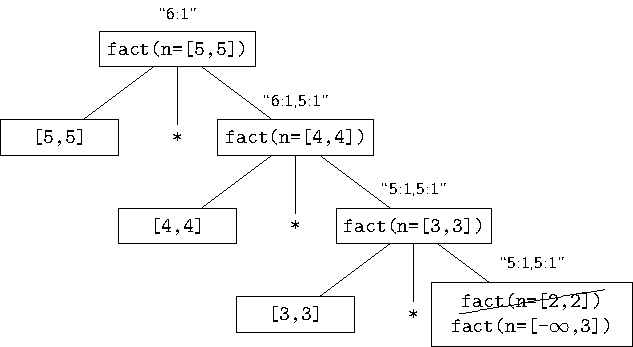
\includegraphics[width=0.8\textwidth]{scheme-generator/generated/example-fun-rec-hierarchy-1.pdf}
    \caption{Prima parte}
    \label{fig:realizzazione:fun-hierarchy-1}
\end{figure}

A questo punto dobbiamo controllare se abbiamo \emph{raggiunto il fixpoint}, cioè se l'ambiente precedente al widening (con $n=[3,3]$) e quello del widening (con $n = [-\infty, 3]$) sono uguali. Non lo sono, quindi continuo l'esecuzione.

Questa chiamata porta ad avere due diramazioni: una ritorna il valore $[1,1]$ ed un altra continua ricorsivamente. Il valore di ritorno viene \emph{salvato} all'interno dell'ambiente dell'istruzione dell'ultima chiamata a funzione con la call string corrente. Ora, quando incontreremo una chiamata a funzione già calcolata (fixpoint) ritorneremo questo valore al posto che eseguire ancora la funzione. Questa parte di esecuzione è visibile in Figura~\ref{fig:realizzazione:fun-hierarchy-2}.

\begin{figure}[htbp]
    \centering
    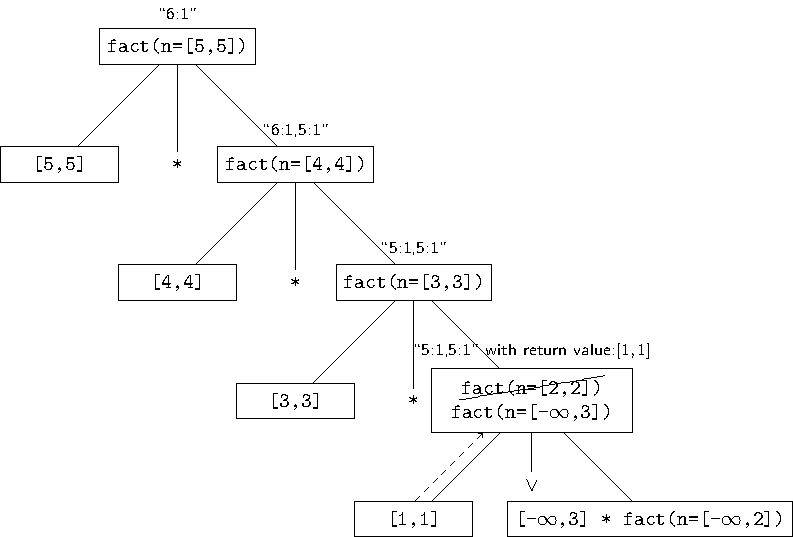
\includegraphics[width=0.8\textwidth]{scheme-generator/generated/example-fun-rec-hierarchy-2.pdf}
    \caption{Seconda parte}
    \label{fig:realizzazione:fun-hierarchy-2}
\end{figure}

L'altra diramazione porta alla chiamata ricorsiva di \texttt{fact}. La call string dopo l'approssimazione è sempre \textsf{``5:1,5:1"}. Applichiamo il widening dei due ambienti, $n$ prende il valore $[-\infty,3]\nabla[-\infty,2]=[-\infty,3]$. Abbiamo raggiunto il fixpoint quindi \emph{non continuiamo l'esecuzione} ma la blocchiamo. Ritorniamo il valore di ritorno associato all'ambiente, che in questo caso è $[1,1]$.  Questa parte di esecuzione è visibile in Figura~\ref{fig:realizzazione:fun-hierarchy-3}.

\begin{figure}[htbp]
    \centering
    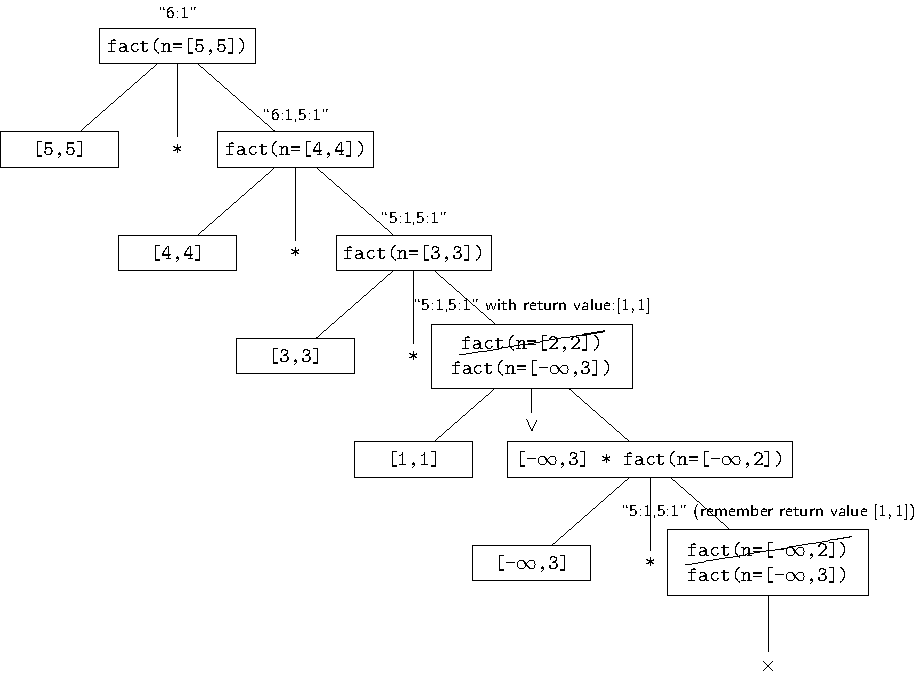
\includegraphics[width=0.8\textwidth]{scheme-generator/generated/example-fun-rec-hierarchy-3.pdf}
    \caption{Terza parte}
    \label{fig:realizzazione:fun-hierarchy-3}
\end{figure}

Ora che ho finito l'esecuzione risalgo l'albero di chiamate ritornando i valori richiesti ai chiamanti. Il risultato finale di \texttt{fact(5)} è un numero compreso nell'intervallo $[-\infty,180]$, coerente col vero valore $5!=120$. L'esecuzione di quest'ultimo step è visibile in Figura~\ref{fig:realizzazione:fun-hierarchy-4}.

\begin{figure}[htbp]
    \centering
    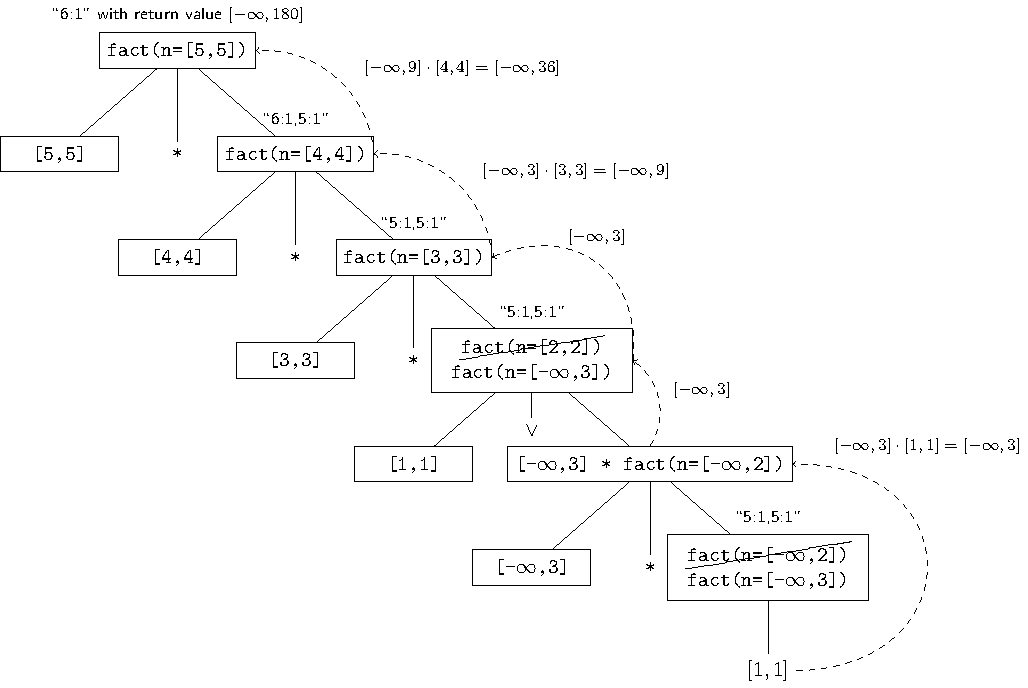
\includegraphics[width=0.8\textwidth]{scheme-generator/generated/example-fun-rec-hierarchy-4.pdf}
    \caption{Completo}
    \label{fig:realizzazione:fun-hierarchy-4}
\end{figure}
